% Script to automatically draw the Quick Ref Sheet

\renewcommand{\arraystretch}{1.2}

\providebool{QRSbool}

\providebool{whiterow}

\newcommand{\QRSrowcolor}{\ifbool{whiterow}{\global\boolfalse{whiterow}}{\rowcolor{black!15}\global\booltrue{whiterow}}}

\newcommand{\QRSstarttab}[1]{%
	\noindent%
	\setlength{\tabcolsep}{2pt}%
	\begin{tabular}{@{}cp{3.2cm}M{\profilecellsize}@{}M{\profilecellsize}@{}M{\profilecellsize}@{}M{\profilecellsize}@{}M{\profilecellsize}@{}M{\profilecellsize}@{}M{\profilecellsize}@{}M{\profilecellsize}@{}M{\profilecellsize}}%

	& \textbf{#1} & \labels@M & \labels@WS & \labels@BS & \labels@S & \labels@T & \labels@W & \labels@I & \labels@A & \labels@Ld%
}%

\newcommand{\QRSclosetab}{\end{tabular}\smallskip}%

\newcommand{\QRSlogowidth}{0.4cm}

\newcommand{\QRSprintline}[4]{%
	\tabularnewline%
	\ifnumequal{\rowmulti}{1}{\QRSrowcolor}{}%
	\DTLifeq*{\rowcategory}{\labels@lords}{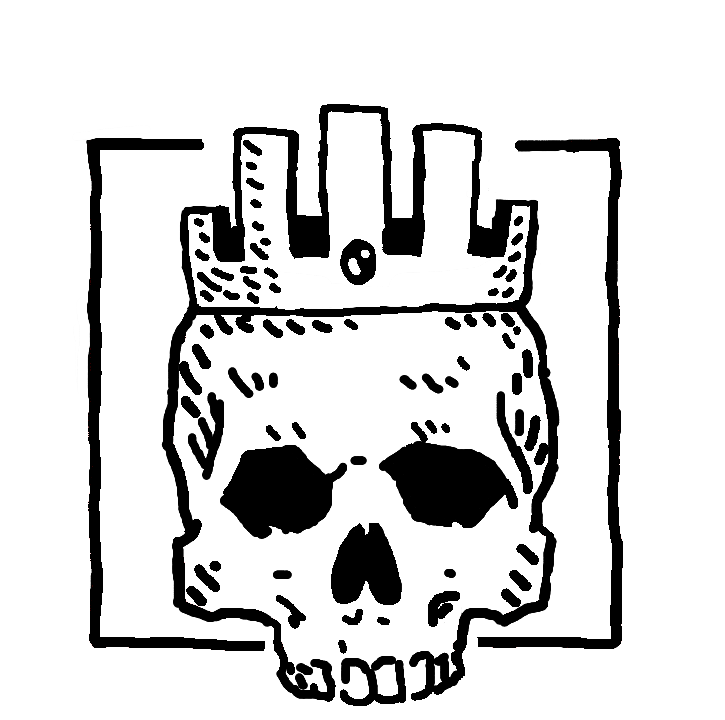
\includegraphics[align=c, width=\QRSlogowidth]{../Layout/pics/logo_lord.png}}{}%
	\DTLifeq*{\rowcategory}{\labels@heroes}{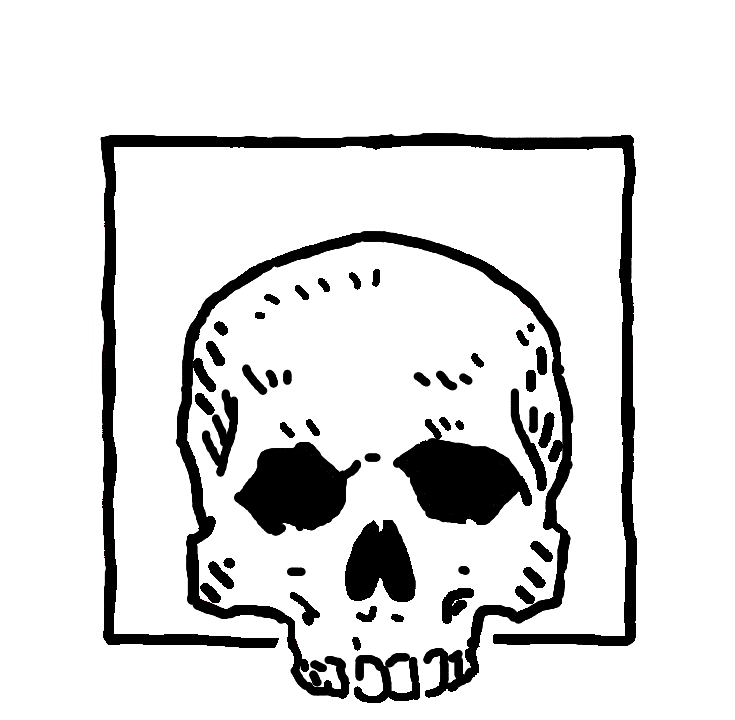
\includegraphics[align=c, width=\QRSlogowidth]{../Layout/pics/logo_hero.png}}{}%
	\DTLifeq*{\rowcategory}{\labels@coreunits}{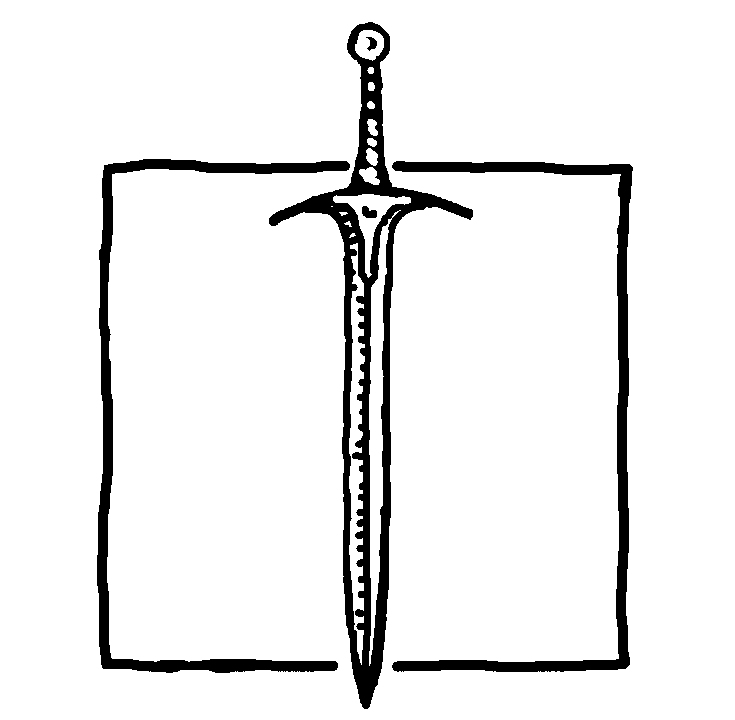
\includegraphics[align=c, width=\QRSlogowidth]{../Layout/pics/logo_core.png}}{}%
	\DTLifeq*{\rowcategory}{\labels@specialunits}{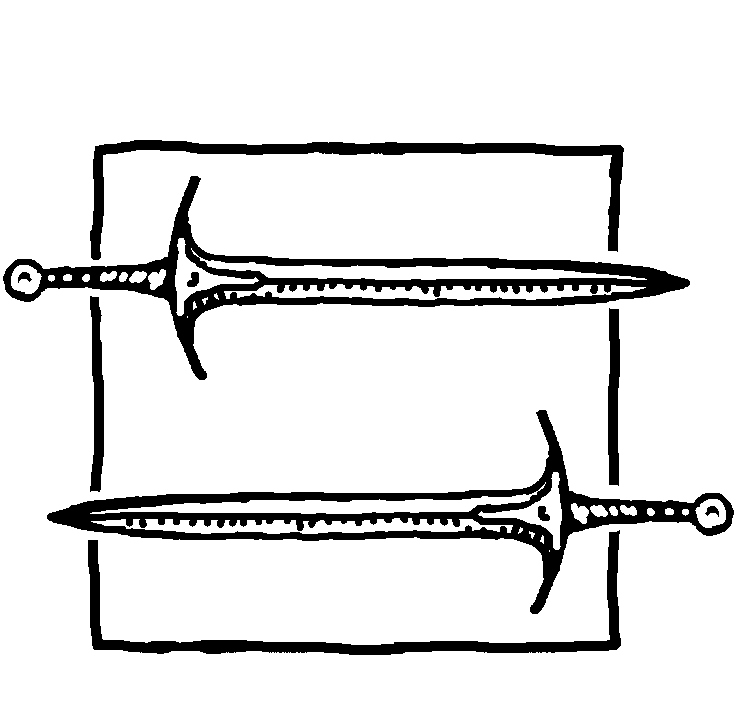
\includegraphics[align=c, width=\QRSlogowidth]{../Layout/pics/logo_special.png}}{}%
	\DTLifeq*{\rowcategory}{\labels@rareunits}{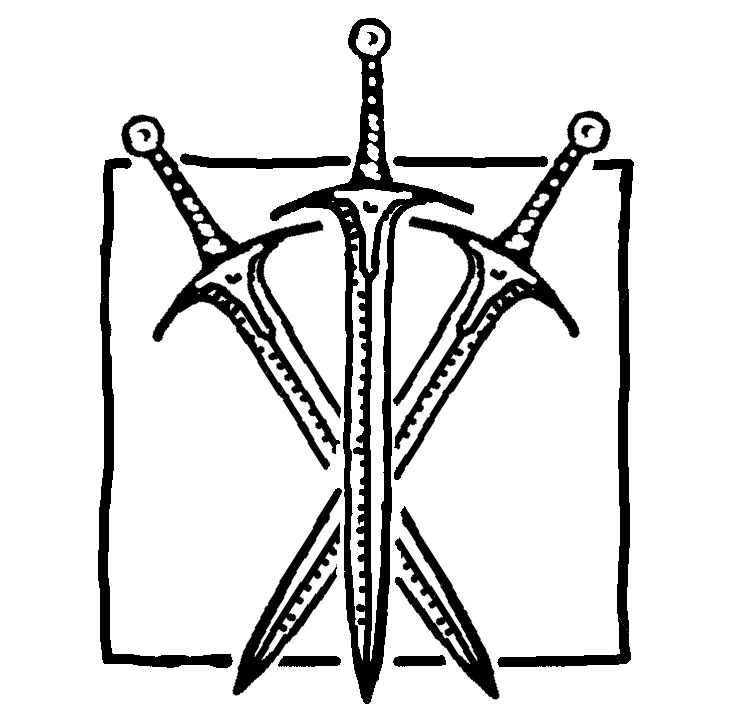
\includegraphics[align=c, width=\QRSlogowidth]{../Layout/pics/logo_rare.png}}{}%
	\DTLifeq*{\rowcategory}{\labels@mounts}{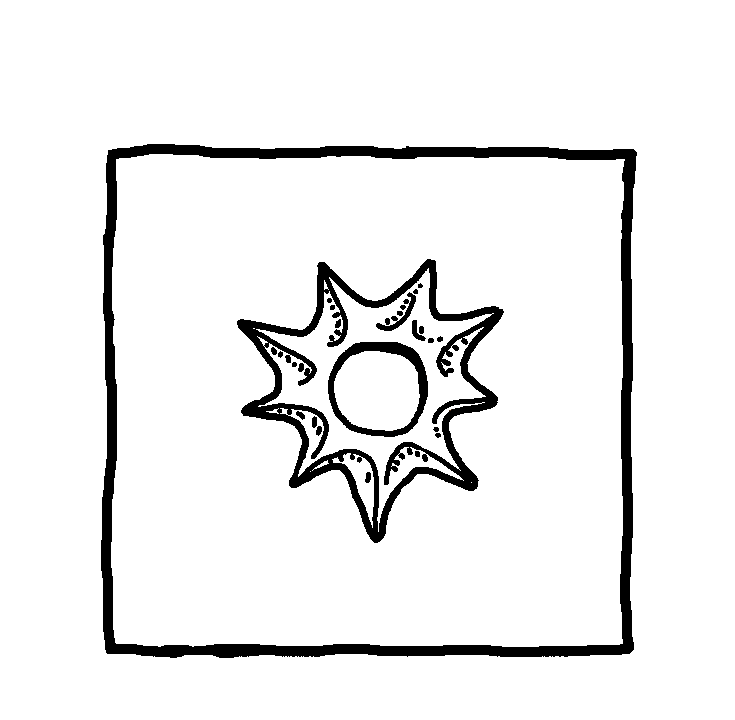
\includegraphics[align=c, width=\QRSlogowidth]{../Layout/pics/logo_mount.png}}{}%
	&%
	\ifnumequal{\rowmulti}{1}{%no Multiprofile
		\rowname%
		\expandafter\parselist\expandafter{\rowprofile}{\locallists@profileslist}%
		\forlistloop{\QRSmonoprofile}{\locallists@profileslist}%
	}{% Multiprofile
		\rowname &&&&&&&&&%
		\expandafter\parselist\expandafter{\rowprofile}{\locallists@profileslist}%
		\forlistloop{\QRSmultiprofile}{\locallists@profileslist}%
	}%
}

\newcommand{\QRSmultiprofile}[1]{%
	\tabularnewline%
	\QRSrowcolor{}&%
	\splitatinf{#1}\local@unitname\local@unitprofile%
	- \local@unitname \expandafter\caraclist\expandafter{\local@unitprofile}%
}%

\newcommand{\QRSmonoprofile}[1]{%
	\splitatinf{#1}\local@unitname\local@unitprofile%
	\expandafter\caraclist\expandafter{\local@unitprofile}%
}%

\newcommand{\QRSprinttab}[1]{%
	\global\booltrue{whiterow}%
	\DTLforeach*[#1]%
	{profiles}{\rowname=name, \rowtrooptype=trooptype, \rowcategory=category, \rowprofile=profile, \rowmulti=multipleprofile}{%
      		\QRSprintline{\rowname}{\rowcategory}{\rowprofile}{\rowmulti}%
	}%
}%

\providebool{QRSisempty}
\global\boolfalse{QRSisempty}%

\newcommand{\QRScheckifempty}[1]{%
	\global\booltrue{QRSisempty}%
	\DTLforeach*[#1]%
	{profiles}{\rowname=name, \rowtrooptype=trooptype, \rowcategory=category, \rowprofile=profile, \rowmulti=multipleprofile}{%
		\global\boolfalse{QRSisempty}\dtlbreak%
	}%
}%

\newcommand{\QRSifnotempty}[1]{%
	\ifbool{QRSisempty}{}{#1}%
}%

\begin{multicols}{2}

\QRScheckifempty{%
	\DTLiseq{\rowcategory}{\labels@lords}\or\DTLiseq{\rowcategory}{\labels@heroes}%
}%
\QRSifnotempty{%
	\QRSstarttab{\characters}%
	\QRSprinttab{%
		\DTLiseq{\rowcategory}{\labels@lords}\or\DTLiseq{\rowcategory}{\labels@heroes}%
	}%
	\QRSclosetab{}%
}%

\QRScheckifempty{%
	\DTLiseq{\rowtrooptype}{\infantry}\and\not\DTLiseq{\rowcategory}{\labels@heroes}\and\not\DTLiseq{\rowcategory}{\labels@lords}%
}%
\QRSifnotempty{%
	\QRSstarttab{\infantry}%
	\QRSprinttab{%
		\DTLiseq{\rowtrooptype}{\infantry}\and\not\DTLiseq{\rowcategory}{\labels@heroes}\and\not\DTLiseq{\rowcategory}{\labels@lords}%
	}% 
	\QRSclosetab{}%
}% 

\QRScheckifempty{%
	\DTLiseq{\rowtrooptype}{\monstrousinfantry}\and\not\DTLiseq{\rowcategory}{\labels@heroes}\and\not\DTLiseq{\rowcategory}{\labels@lords}%
}%
\QRSifnotempty{%
	\QRSstarttab{\monstrousinfantry}%
	\QRSprinttab{%
		\DTLiseq{\rowtrooptype}{\monstrousinfantry}\and\not\DTLiseq{\rowcategory}{\labels@heroes}\and\not\DTLiseq{\rowcategory}{\labels@lords}%
	}% 
	\QRSclosetab{}%
}% 

\QRScheckifempty{%
	\DTLiseq{\rowtrooptype}{\warbeast}\and\not\DTLiseq{\rowcategory}{\labels@heroes}\and\not\DTLiseq{\rowcategory}{\labels@lords}%
}%
\QRSifnotempty{%
	\QRSstarttab{\warbeasts}%
	\QRSprinttab{%
		\DTLiseq{\rowtrooptype}{\warbeast}\and\not\DTLiseq{\rowcategory}{\labels@heroes}\and\not\DTLiseq{\rowcategory}{\labels@lords}%
	}% 
	\QRSclosetab{}%
}% 

\QRScheckifempty{%
	\DTLiseq{\rowtrooptype}{\monstrousbeast}\and\not\DTLiseq{\rowcategory}{\labels@heroes}\and\not\DTLiseq{\rowcategory}{\labels@lords}%
}%
\QRSifnotempty{%
	\QRSstarttab{\monstrousbeasts}%
	\QRSprinttab{%
		\DTLiseq{\rowtrooptype}{\monstrousbeast}\and\not\DTLiseq{\rowcategory}{\labels@heroes}\and\not\DTLiseq{\rowcategory}{\labels@lords}%
	}% 
	\QRSclosetab{}%
}% 

\QRScheckifempty{%
	\DTLiseq{\rowtrooptype}{\cavalry}\and\not\DTLiseq{\rowcategory}{\labels@heroes}\and\not\DTLiseq{\rowcategory}{\labels@lords}%
}%
\QRSifnotempty{%
	\QRSstarttab{\cavalry}%
	\QRSprinttab{%
		\DTLiseq{\rowtrooptype}{\cavalry}\and\not\DTLiseq{\rowcategory}{\labels@heroes}\and\not\DTLiseq{\rowcategory}{\labels@lords}%
	}%
	\QRSclosetab{}%
}% 

\QRScheckifempty{%
	\DTLiseq{\rowtrooptype}{\monstrouscavalry}\and\not\DTLiseq{\rowcategory}{\labels@heroes}\and\not\DTLiseq{\rowcategory}{\labels@lords}%
}%
\QRSifnotempty{%
	\QRSstarttab{\monstrouscavalry}%
	\QRSprinttab{%
		\DTLiseq{\rowtrooptype}{\monstrouscavalry}\and\not\DTLiseq{\rowcategory}{\labels@heroes}\and\not\DTLiseq{\rowcategory}{\labels@lords}%
	}%
	\QRSclosetab{}%
}% 

\QRScheckifempty{%
	\DTLiseq{\rowtrooptype}{\chariot}\and\not\DTLiseq{\rowcategory}{\labels@heroes}\and\not\DTLiseq{\rowcategory}{\labels@lords}%
}%
\QRSifnotempty{%
	\QRSstarttab{\chariots}%
	\QRSprinttab{%
		\DTLiseq{\rowtrooptype}{\chariot}\and\not\DTLiseq{\rowcategory}{\labels@heroes}\and\not\DTLiseq{\rowcategory}{\labels@lords}%
	}%
	\QRSclosetab{}%
}% 

\QRScheckifempty{%
	\DTLiseq{\rowtrooptype}{\monster}\and\not\DTLiseq{\rowcategory}{\labels@heroes}\and\not\DTLiseq{\rowcategory}{\labels@lords}%
}%
\QRSifnotempty{%
	\QRSstarttab{\monsters}%
	\QRSprinttab{%
		\DTLiseq{\rowtrooptype}{\monster}\and\not\DTLiseq{\rowcategory}{\labels@heroes}\and\not\DTLiseq{\rowcategory}{\labels@lords}%
	}%
	\QRSclosetab{}%
}% 

\QRScheckifempty{%
	\DTLiseq{\rowtrooptype}{\swarm}\and\not\DTLiseq{\rowcategory}{\labels@heroes}\and\not\DTLiseq{\rowcategory}{\labels@lords}%
}%
\QRSifnotempty{%
	\QRSstarttab{\swarms}%
	\QRSprinttab{%
		\DTLiseq{\rowtrooptype}{\swarm}\and\not\DTLiseq{\rowcategory}{\labels@heroes}\and\not\DTLiseq{\rowcategory}{\labels@lords}%
	}%
	\QRSclosetab{}%
}% 

\end{multicols}



\restoregeometry